\documentclass[12pt]{article}
\usepackage[english]{babel}
\usepackage{tocloft}
\addtolength{\cftsecnumwidth}{12pt}
\addtolength{\cftsubsecnumwidth}{12pt}
\setlength{\cftsubsecindent}{30pt}
\usepackage{endnotes}
\usepackage{scrextend}
\usepackage[T1]{fontenc}
\usepackage[utf8]{inputenc}
\usepackage{url}
\usepackage{paralist}
\usepackage{array}
\newcolumntype{R}[1]{>{\let\newline\\\arraybackslash\hspace{0pt}}m{#1}}
\usepackage{float}
\usepackage{authblk}
\usepackage{tablefootnote}
\usepackage{todonotes}
\usepackage{lscape}
\usepackage{chronology}
\usepackage{mdframed}
\usepackage{enumitem, amssymb}
\usepackage{graphicx} 
\usepackage{color}
\usepackage{booktabs} 
\usepackage{dcolumn}
\usepackage[defaultfam,tabular,lining]{montserrat} 
\usepackage{mathpazo}
\usepackage{xcolor}
\definecolor{abblue}{RGB}{30,150,186}
\definecolor{abblueD}{RGB}{44,143,159}
\definecolor{aborange}{RGB}{223,109,33}
\usepackage[left=1in,right=1in,top=1in, bottom=1in]{geometry}
\usepackage{background}
\usepackage{multicol}
\usepackage{fancyhdr}
\pagestyle{fancy}
\fancyhf{}
\renewcommand\headrule{}
\fancyhead[L]{\color{gray}\footnotesize{Arab Barometer -- Wave V} \\
	\color{gray}\footnotesize{Country Report}}
\cfoot{\color{gray}\footnotesize{www.arabbarometer.org}}
\rfoot{\color{gray}\footnotesize{ \thepage}}
\usepackage{tocloft}
\renewcommand{\cftsubsecfont}{\hypersetup{linkcolor=gray}}
\usepackage{hyperref}
\hypersetup{colorlinks=false,pdfborder=0 0 0,citebordercolor={0 0 0}}
\renewcommand\thefootnote{\textcolor{gray}{\arabic{footnote}}}

\begin{document}
	\newpage
	\backgroundsetup{
		scale=1,
		color=black,
		opacity=1,
		angle=0,
		contents={%
			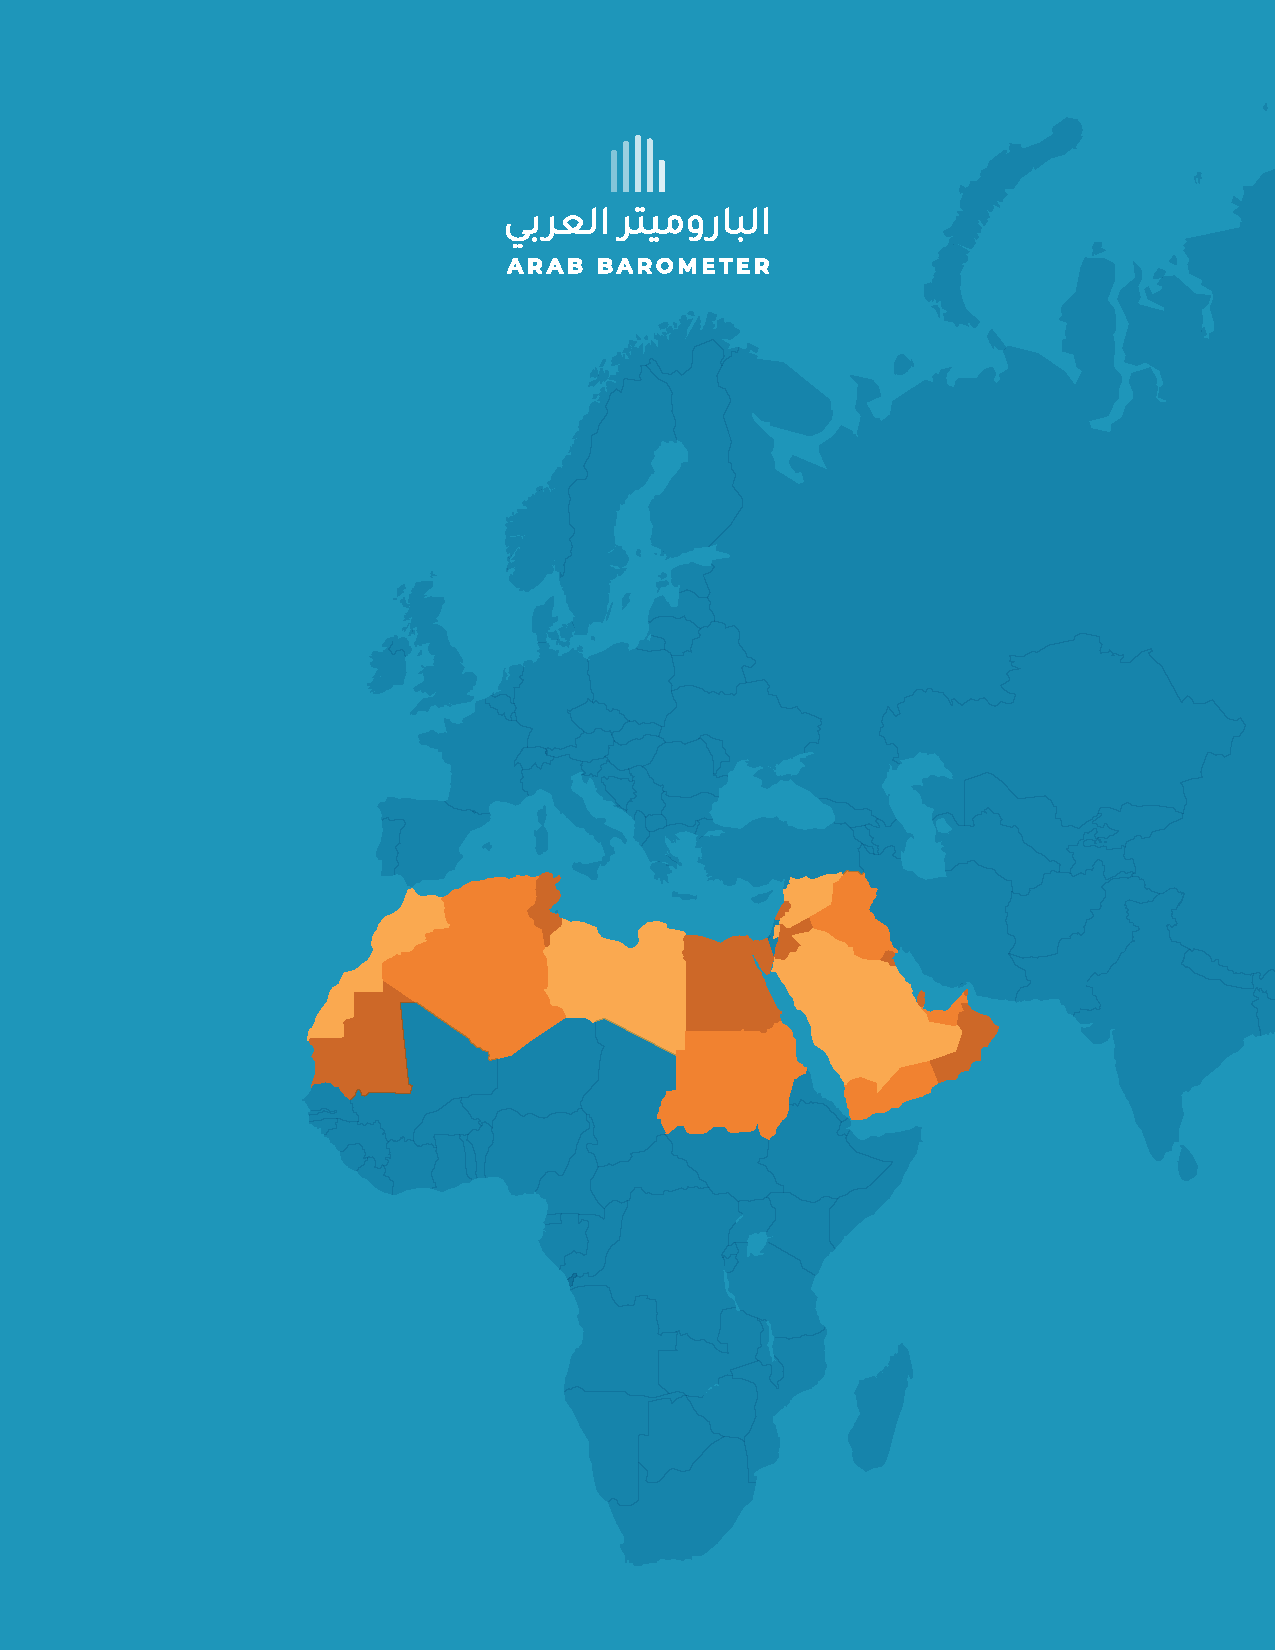
\includegraphics[width=\paperwidth,height=\paperheight]{AB_FrontCover.pdf}
		}%
	}
	\newgeometry{left=1in,right=1in,top=1in, bottom=1in}
	\pagestyle{empty} 
	\vspace*{2in}
	\begin{center}
		\color{white}\Huge\textbf{Arab Barometer V} \\
		\vspace*{0.5in}
		\color{white}\LARGE\textbf{Morocco Country Report} \\
		\vspace*{4in}
		\color{white}\large\textbf{2019} \\
	\end{center}
	%%%%%%%%%%%%%%%%%%%%%%%%%%%%
	\newpage\backgroundsetup{contents={}}
	\color{gray}
	\color{gray}
	\pagestyle{fancy}
%%%%%%%%%%%%%%%%%%%%%%%%%%%%%%%%%%%
	\pagebreak
	\section*{Executive summary}
	Morocco is a country split in two by generations. The older generation of Moroccans retains confidence in the country's institutions, while younger Moroccans are growing increasingly frustrated by the lack of available economic and political opportunities. Morocco remains stable, but the undercurrent of discontent among the country's youth does not auger well, especially amid the turmoil sweeping a number of countries in the region. A key government priority should be to address the needs and concerns of this rising generation.\\
	
	\noindent Viewed in the eyes of the public, significant challenges facing Morocco include the economy and the quality of public services. The vast majority of Moroccans also say corruption is found in state institutions, although the percentage has declined in recent years, perhaps reflecting efforts to stem this problem.\\
	
	\noindent The inability to solve these longstanding problems is also having consequences for the government.  Levels of trust in political institutions are low and falling, particularly among the youth generation. However, trust remains high in the army, police and judiciary.\\
	
	\noindent These challenges are driving nearly half of Moroccans to consider emigrating from their homeland, including seven-in-ten youth between the ages of 18 and 29. Critically, those who want to emigrate also tend to be those with higher levels of education, which could be future leaders of the country. Likely a product of Morocco's proximity, most want to seek opportunities in Europe, although a majority say they would only leave Morocco if they received legal permission.\\
	
	\noindent The younger generation is also turning away from religion, at least relative to the older generations. Just one-in-four of those ages 18-29 describe themselves are religious compared with two-thirds of those 60 and older. Similarly, support for political Islam is in sharp decline in Morocco, especially among youth.\\
	
	\noindent These are among the key findings from a nationally representative public opinion survey conducted in Morocco by the Arab Barometer in October-December 2018. The survey conducted 2,400 face-to-face interviews in the respondent's place of residence has a margin of error of $\pm$2 percent and had a response rate of 55 percent.
	\pagebreak
%%%%%%%%%%%%%%%%%%%%%%%%%%%%%%
%%%%%  

\section*{Economic Conditions}

	Moroccans are divided on the main challenge facing their country. A plurality (26 percent) say economic issues are the primary issue, followed by the quality of public services (23 percent) and corruption (9 percent). Notably, a large percentage of Moroccans cite other problems (32 percent), including the use of drugs and marginalization.\\
	
	\begin{center}
	{\textbf{What is the most important challenge facing your country today?}}\\
	\emph{\% saying this is the most important challenge.}
	\begin{figure}[H]
		\centering
		\includegraphics[width=11cm]{Q2061A_overall.pdf}
	\end{figure}
	\end{center}

	\noindent Overall, just over a third (36 percent) rate the economy as good or very good, which is a dramatic decline from 2016 (-30 points). In part, this change is likely linked with the end of extended high in world prices for phosphates which collapsed in 2016-7.\footnote{\color{gray}Morocco is the world's third leading exporter of phosphates. The price of phosphates collapsed beginning in 2016, falling by more than a third by late 2017.} Instead, 2016 appears to be a significant outlier, with ratings of the economy virtually the same in 2019 as in 2013 (37 percent).
	
	\pagebreak
		\begin{center}
		{\textbf{How would you evaluate the current economic situation in your country?}}\\
		\emph{\% saying the current economy is very good or good.}
		\end{center}
	\begin{figure}[H]
		\hspace{-1cm}\begin{minipage}{0.5\linewidth}
			\begin{figure}[H]
				\centering
				\includegraphics[width=6.5cm]{R101_age.pdf} 
			\end{figure}
		\end{minipage}
		\begin{minipage}{0.4\linewidth}
			\begin{figure}[H]
				\includegraphics[width=6.5cm]{R101_education.pdf}
			\end{figure}
			\end{minipage}
	\end{figure}
	
	\noindent Views of the economy are strongly linked with age.  Although roughly half (53 percent) of those ages 60 and older say the economy is good or very good, only half of those ages 18 to 29 say the same (27 percent). Notably, economic perceptions do not vary dramatically by level of education -- 41 percent of those with a basic education say the economy is good compared with 38 percent of those with a university degree. However, those with only a high school degree are somewhat less likely to rate the economy positively (28 percent).
	
	\noindent Only three-in-ten expect economic conditions to improve in the near future, which is a dramatic reversal from previous surveys. Since 2006, at least half of Moroccans said they expected economic conditions to get better. Again, youth are particularly pessimistic, with only a quarter of those ages 18-29 saying the economic will get better compared with 41 percent of those ages 60 and older.
	
	\pagebreak
		\begin{center}
		{\textbf{What do you think the economic situation in your country will be in the next few years (2-3 years) compared to the current situation?}}\\
		\emph{\% saying the economy will  be much or somewhat better in 2-3 years.}
		\begin{figure}[H]
			\centering
			\includegraphics[width=11cm]{q102trend.pdf}
		\end{figure}
	\end{center}

\section*{Corruption}

	\noindent Corruption remains a significant challenge in Morocco, at least in the views of its citizens. Seven-in-ten (71 percent) say that corruption is found within state institutions to a large or medium extent. Notably, there is some good news -- this percentage has declined slowly but steadily since 2013, falling from 83 percent to 71 percent.\\
	
	\noindent However, again there is a significant generational divide. Among those ages 18-29, 81 percent say there is corruption in state institutions, which is 32 points more than those who are ages 60 and above (49 percent). Perceptions of corruption are also linked by education, where those with a secondary or university degree are also more likely than those with a basic level of education to say there is corruption.
	
	\pagebreak
	\begin{center}
		{\textbf{To what extent do you think that there is corruption within the national state agencies and institutions in your country?}}\\
		\emph{\% saying to a large or medium extent.}
	\end{center}
	\begin{figure}[H]
		\hspace{-1cm}\begin{minipage}{0.5\linewidth}
			\begin{figure}[H]
				\centering
				\includegraphics[width=6.5cm]{R210_age.pdf} 
			\end{figure}
		\end{minipage}
		\begin{minipage}{0.4\linewidth}
			\begin{figure}[H]
				\includegraphics[width=6.5cm]{R210_education.pdf}
			\end{figure}
		\end{minipage}
	\end{figure}

	\noindent Despite the fact that most say there is significant corruption, relatively few believe that the government is taking significant steps to tackle the problem. Slightly more than a third (36 percent) say the government is cracking down on corruption to a great or medium extent, which is down 14 points since 2016, but similar to 2013 (33 percent).
	
	\begin{center}
		{\textbf{In your opinion, to what extent is the national government working to crackdown on corruption?}}\\
		\emph{\% saying to a large or medium extent.}
		\begin{figure}[H]
			\centering
			\includegraphics[width=11cm]{q211trend.pdf}
		\end{figure}
	\end{center}
	
	\noindent Youth are the least likely to believe the state is serious about tackling corruption.  Just a quarter (26 percent) of those ages 18 to 29 say the government is doing so, while those 50 and older are 30 points more likely to say the same. Meanwhile, nearly half of those with a basic level of education (45 percent) think the government is addressing the issue, compared with just 32 percent of those with a university degree and 28 percent of those with a secondary degree.\\
	
	\noindent Perceptions of corruption at the local level are somewhat less -- half (46 percent) say that hardly any or few officials at the local level are engaged in corruption. Again, perceptions vary drastically by age with 36 percent of youth ages 18-29 holding this view compared with 68 percent of those over 60 years who say the same.\\
	
	\noindent The use of bribes remains a common part of life in Morocco. Nearly two-thirds (64 percent) say that bribes are necessary (30 percent) or highly necessary (34 percent) to receive better health care services. Meanwhile, 46 percent say the same about better educational services. Again, generational differences stand out with younger Moroccans being far more likely to say bribes are necessary than those who are older.
	
		\begin{center}
		{\textbf{In your opinion, to what extent do you think it is necessary to pay rashwa to a civil servant of your country to receive better health care services?}}\\
		\emph{\% saying highly or somewhat necessary.}
		\begin{figure}[H]
			\centering
			\includegraphics[width=11cm]{R211C_age.pdf}
		\end{figure}
	\end{center}

\section*{Trust in Government}

	\noindent Moroccans are significantly less likely to trust the government than in previous waves. Just three-in-ten have a great deal or quite a lot of trust in the government now compared with previous surveys conducted in 2006, 2013 and 2016 when roughly four-in-ten trusted the government.
	
	\begin{center}
		{\textbf{I'm going to name a number of institutions. For each one, please tell me how much trust you have in them: Government}}\\
		\emph{\% saying they have a great deal or quite a lot of trust.}
		\begin{figure}[H]
			\centering
			\includegraphics[width=11cm]{q2011trend.pdf}
		\end{figure}
	\end{center}
	
	\noindent Trust is particularly low among youth and better educated. Just 17 percent of those ages 18 to 29 trust the government, which is three times fewer than those who are sixty or older. Similarly, those with a basic level of education (37 percent) are significantly more likely to have confidence in the government than those with a university degree (24 percent) or secondary degree (19 percent).
	
		\pagebreak
	\begin{center}
		{\textbf{I'm going to name a number of institutions. For each one, please tell me how much trust you have in them: Government}}\\
		\emph{\% saying they have a great deal or quite a lot of trust.}
	\end{center}
	\begin{figure}[H]
		\hspace{-1cm}\begin{minipage}{0.5\linewidth}
			\begin{figure}[H]
				\centering
				\includegraphics[width=6.5cm]{R201A_1_age.pdf} 
			\end{figure}
		\end{minipage}
		\begin{minipage}{0.4\linewidth}
			\begin{figure}[H]
				\includegraphics[width=6.5cm]{R201A_1_education.pdf}
			\end{figure}
		\end{minipage}
	\end{figure}

	\noindent Only one-in-five (21 percent) have a great deal or some trust in parliament, compared with a quarter (26 percent) who say little trust and 46 percent who say no trust. Trust has not changed substantially since 2006 when 25 percent had at least some confidence in the legislature. As with other measures, those who are younger tend to have lower levels of trust, including just 13 percent of those ages 18-29 compared to 38 percent of those 60 and older.
	
		\begin{center}
		{\textbf{I'm going to name a number of institutions. For each one, please tell me how much trust you have in them: Parliament}}\\
		\emph{\% saying they have a great deal or quite a lot of trust.}
		\begin{figure}[H]
			\centering
			\includegraphics[width=11cm]{q2013trend.pdf}
		\end{figure}
	\end{center}

	\noindent A similar percentage have confidence in political parties (18 percent). Although low, this percentage represents a substantial increase from 2016 (+8 points). Those over 60 years are about three times more likely to trust political parties than those ages 18-29 (35 percent vs. 11 percent).\\
	
	\noindent Levels of trust are significantly higher in institutions that are tasked with ensuring law and order. The vast majority (78 percent) trust the army, while two-thirds also trust the police. These percentages are somewhat lower than in other MENA countries, and youth are significantly less likely to have confidence in both institutions than are those who are older.
	
		\begin{center}
		{\textbf{I'm going to name a number of institutions. For each one, please tell me how much trust you have in them: The judiciary}}\\
		\emph{\% saying they have a great deal or quite a lot of trust.}
		\begin{figure}[H]
			\centering
			\includegraphics[width=11cm]{q2012trend.pdf}
		\end{figure}
	\end{center}
	
	\noindent Moreover, six-in-ten trust the judiciary, which is a dramatic increase in recent years. In 2006 just 37 percent trusted the judiciary while 45 percent did in 2016. Majorities across all ages have confidence in the judiciary, although older Moroccans are more likely to trust it than younger ones. There is a 24-point gap between those who are ages 18-29 and those who are sixty and older (54 percent vs. 78 percent).

\section*{Migration}

	\noindent Moroccans are significantly more likely to want to emigrate than they were in 2016. Now, fully 44 percent say they want to leave their homeland, which is a 17-point increase since the 2016 survey. Notably, this also reverses a long-standing trend where the percentage wanting to emigrate was decreasing from 52 percent in 2006 to 27 percent in 2016.
	
		\begin{center}
		{\textbf{Have you ever thought about emigrating from your country?}}\\
		\emph{\% saying they thought about emigrating.}
		\begin{figure}[H]
			\centering
			\includegraphics[width=11cm]{q104trend.pdf}
		\end{figure}
	\end{center}
	
	\noindent Migration is strongly linked with age -- fully 70 percent of those ages 18-29 want to leave Morocco, compared with half (49 percent) of those 30-39, 22 percent 40-49 and fewer than 10 percent who are fifty or older. Morocco is at significant risk of brain drain as well as more than sixty percent of those with a secondary or university degree want to leave their homeland. Notably, men are far more likely to want to emigrate than women (61 percent vs. 28 percent).
	
	\pagebreak
	\begin{center}
		{\textbf{Have you ever thought about emigrating from your country?}}\\
		\emph{\% saying they thought about emigrating.}
	\end{center}
	\begin{figure}[H]
		\hspace{-1cm}\begin{minipage}{0.5\linewidth}
			\begin{figure}[H]
				\centering
				\includegraphics[width=6.5cm]{R104_age.pdf} 
			\end{figure}
		\end{minipage}
		\begin{minipage}{0.4\linewidth}
			\begin{figure}[H]
				\includegraphics[width=6.5cm]{R104_education.pdf}
			\end{figure}
		\end{minipage}
	\end{figure}
	
	\noindent The reasons that Moroccans want to emigrate vary. The most common one is because of economic considerations (50 percent), followed by educational opportunities (15 percent), to reunite with family (14 percent), and corruption (6 percent). Meanwhile, 15 percent name another reason, some of which include concerns about drugs or feeling marginalized.
	
			\begin{center}
		{\textbf{People want to emigrate for different reasons. Why have you thought about emigrating?}}
%		\emph{\% saying they thought about emigrating.}
		\begin{figure}[H]
			\centering
			\includegraphics[width=9cm]{Q104A_overall.pdf}
		\end{figure}
	\end{center}

	\noindent Potential migrants are by far most likely to look to go to Europe with nearly two-thirds (64 percent) citing Europe as their preferred destination. Meanwhile, 12 percent want to go to the U.S. or Canada while 5 percent want to go to a GCC country and 10 percent want to go to a non-GCC Arab country. Additionally, 26 percent prefer another destination including sub-Saharan Africa, Asia or Latin America. Notably, a majority of potential migrants (56 percent) say they would \textit{not} migrate illegally compared with 38 percent who say they would consider leaving even if they lacked the necessary papers.

		\begin{center}
		{\textbf{Which region are you thinking of emigrating to?}}\\
		%		\emph{\% saying they thought about emigrating.}
		\begin{figure}[H]
			\centering
			\includegraphics[width=11cm]{Q104B_overall.pdf}
		\end{figure}
	\end{center}

\section*{Religious Belief}
	
	\noindent Nearly four-in-ten Moroccans say they are religious (38 percent), compared with 44 percent who are somewhat religious and 13 percent identifying as not religious. \\
	
	\noindent Again, the youth generation stands out from the the older generation. Those who are ages 18-29 are more than 40 points less likely to identify as religious compared with those who are 60 or older (24 percent vs. 68 percent). As in many countries, those with a higher level of education are somewhat less likely to be religious; those with a basic education in Morocco are about 20 points more likely to be religious than those with a secondary degree or university education. Women are also more likely to be religious than men (44 percent vs. 31 percent), although notably those in urban and rural areas are equally likely to be religious.
	
		\begin{center}
		{\textbf{In general, would you describe yourself as religious, somewhat religious, or not religious?}}\\
		\emph{\% saying they are religious.}
	\end{center}
	\begin{figure}[H]
		\hspace{-1cm}\begin{minipage}{0.5\linewidth}
			\begin{figure}[H]
				\centering
				\includegraphics[width=6.5cm]{R609_age.pdf} 
			\end{figure}
		\end{minipage}
		\begin{minipage}{0.4\linewidth}
			\begin{figure}[H]
				\includegraphics[width=6.5cm]{R609_education.pdf}
			\end{figure}
		\end{minipage}
	\end{figure}

	\noindent Support for political Islam is also in decline in Morocco. In 2006, nearly six-in-ten (58 percent) said that religious leaders should have say over decisions of government. This percentage has steadily declined falling to just 21 percent in 2018.
	
	\pagebreak
		\begin{center}
		{\textbf{How much do you agree or disagree with each of the following statement? Religious leaders should have influence over government decisions}}\\
		\emph{\% saying they strongly agree or agree.}
		\begin{figure}[H]
			\centering
			\includegraphics[width=11cm]{q6063trend.pdf}
		\end{figure}
	\end{center}
	
	\noindent This decline may be linked to the fact that the younger generation is substantially less likely to want religious figures to have say over government. Just 12 percent of those ages 18-29 and 15 percent of those 30-39 hold this view, compared with a third (34 percent) of those 50-59 and four-in-ten who are 60 and older. Additionally, those who have a basic level of education (30 percent) are more likely to hold this view than those with a secondary (15 percent) or tertiary degree (9 percent).\\
	
	\noindent Among Moroccan Muslims, roughly a quarter (27 percent) believe that the law should be entirely (12 percent) or mostly (15 percent) based on the sharia. Instead, a plurality (32 percent) say the law should be based equally on the sharia and the will of the people, while 21 percent say it should be based mostly on the will of the people and 15 percent say it should be entirely based on what the people prefer. Support for making laws mostly or entirely based on the sharia has declined since 2016, falling by 9 points.\\
	
	\noindent Younger and better educated Moroccan Muslims are less likely to favor laws based on the sharia. Only 17 percent of those ages 18-29 hold this view compared with nearly half (47 percent) of those 60 and older. Meanwhile, 37 percent of those with a basic education say the law should at least mostly follow the sharia compared with 20 percent of those with a secondary degree and 13 percent of those with a university degree.
			
	\pagebreak
	\begin{center}
		{\textbf{From your point of view, should the laws of our country be...?}}\\
		\emph{\% saying entirely or mostly on the sharia.}
	\end{center}
	\begin{figure}[H]
		\hspace{-1cm}\begin{minipage}{0.5\linewidth}
			\begin{figure}[H]
				\centering
				\includegraphics[width=6.5cm]{R605_age.pdf} 
			\end{figure}
		\end{minipage}
		\begin{minipage}{0.4\linewidth}
			\begin{figure}[H]
				\includegraphics[width=6.5cm]{R605_education.pdf}
			\end{figure}
		\end{minipage}
	\end{figure}


	
%%%%%%%%%%%%%%%%%%%%%%%%%%%%%%
%%%%%  
%%%%%%%%%%%%%%%%%%%%%%%%%%%%%%%%%%%  
\newpage
\pagestyle{empty}
\backgroundsetup{
	scale=1,
	color=black,
	opacity=1,
	angle=0,
	contents={%
		\includegraphics[width=\paperwidth,height=\paperheight]{AB_BackCover.pdf}
	}%
}
\newgeometry{left=1.5in,right=1.5in,top=1in, bottom=1in}
\pagestyle{empty} 
\vspace*{1in}
\centering
\textbf {\LARGE \color{white} 	\href{http://www.arabbarometer.org/about}{About Arab Barometer}} \\
\vspace*{0.2in}
	\normalsize \color{white}{The Arab Barometer is a nonpartisan research network that provides insights into the social, political, and economic attitudes and values of ordinary citizens across the Arab world. \\
	\vspace*{0.2in}
	We have been conducting rigorous, and nationally representative face-to-face public opinion surveys on probability samples of the adult populations across the Arab world since 2006. The margin of error is $\pm$3 percent. \\
	\vspace*{0.2in}
	The Arab Barometer is the largest repository of publicly available data on the views of men and women in the MENA region. Our findings give a voice to the needs and concerns of Arab publics.  \\
%	\vspace*{0.2in}	
%	Through 2019, the Arab Barometer has conducted 49 national surveys over five waves including more than 74,000 interviews in 14 Arab countries. \\
	\vspace*{4.1in}	
	\begin{tabular}{R {2.2in} R {2in} R {2in}}
		\Huge \color{abblue}{
			\href{http://www.arabbarometer.org}{..........} }&
		\Huge \color{abblueD}{\href{http://www.facebook.com/arabbarometer/}{..........} }&	
		\Huge \color{abblue}{
			\href{https://twitter.com/arabbarometer}{..........}}\\
	\end{tabular}
\end{document}

	